
\rule{\textwidth}{0.4pt} 
\class{AirQualityData}
public abstract class AirQualityData

\begin{minipage}{0.3\textwidth}
    \begin{figure}[H]
        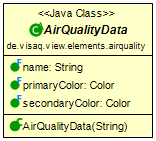
\includegraphics[scale = 0.6]{media/frontend/view/de.view.elements.airquality/AirQualityData_Class.png}
    \end{figure}
    \end{minipage} \hfill
    \begin{minipage}{0.6\textwidth}
Objekt welches dafür verwendet wird die unterschiedlichen Farbschemata für die Legenden darzustellen.
\end{minipage}

Attribute:
\begin{itemize} 
    \item \emph{public static final String name} Der Name der angezeigten Luftqualitätsdata in der Navigationsbar
    \item \emph{public final Color primaryColor} Die Primärfarbe des Typen 
	\item \emph{public final Color secondaryColor} Die Sekundärfarbe des Typen
\end{itemize}
Methoden:
\begin{itemize} 
    \item \emph{public AirQualityData(String name)} Konstruktor für die AirQualityData
\end{itemize}

